\chapter[A shim Layer for persistent memory]{A shim layer for persistent memory}

As we have discussed, the release of Intel Optane PMM opens a major opportunity for serverless storage services. This memory technology provides a unique combination of affordable larger capacity, high-performance, and support for data persistence \cite{IntelOp15:online}. When configured in App-Direct mode, the Optane DIMM and DRAM DIMMs act as independent memory resources under direct load/store control of the applications. This allows the Optane PMM capacity to be used as byte-addressable persistent memory that is mapped into the system application space and directly accessible by applications. Together, these advantages enable Optane PMM to be used as persistent storage with memory-like speeds.

Unfortunately, the resource contention observed within Optane PMM can impose serious performance and contractual implications for a multi-tenant serverless storage service. Given the hallmark autoscaling features of serverless computing, the memory’s limited ability to handle accesses from multiple threads can degrade the overall system’s performance when workload spikes occur. Furthermore, these storage systems make efficient use of their infrastructure by allowing multiple users, or tenants, to share the physical resources. The performance degradation caused by Optane PMM can lead tenants to experience significant performance variations. The latter inhibits service providers from offering certain service level agreements.

To reduce the contention effect, previous studies recommend limiting the number of threads that access Optane PMM simultaneously. In \cite{yang2020empirical}, Yang et. al they improve the performance of an NVM-aware file system by limiting the number of writer threads that access each Optane DIMM. Similarly, Ribbon \cite{wu2020ribbon} controls the number of threads performing CLF and adjusts this number dynamically at runtime. While this approach provides a viable solution, it introduces management problems for a system administrator of a multi-tenant serverless storage.

Given the complexity of serverless computing workloads, implementing efficient concurrency control mechanisms for optimizing an Optane-based serverless storage service is a challenging task. These challenges are discussed in section 3.1, but in short, service providers have three crucial tasks when implementing these control mechanisms. First, they must provide predictable performance, ensuring that all the SLAs from different workloads are met. Second, they must scale resources transparently to meet the current workload demand. Finally, they must come up with policies that allow their system to adapt quickly to sudden workload shifts. To this end, we propose a solution that takes on these responsibilities from the service providers.

In this work, we present a shim layer that addresses the shortcomings of Intel Optane PMM highlighted above, while meeting the different service level agreements from multiple tenants under shifting workloads. Our shim layer, called NVM Middleware, distinguishes between latency-critical and throughput-oriented workloads and applies different concurrency control mechanisms for each one. This enables the system to reduce the contention on the memory device, as well as the interference among workloads with different service level agreements. In addition, we propose the development of a reinforcement learning agent to adapt the NVM Middleware quickly to changing workloads. The agent takes into account the characteristics and service level agreements and learns from past experiences to scale resources accordingly.


\section{Motivation}
In this section, we discuss the pain points of controlling the number of threads to optimize Optane PMM within a serverless storage service and explain the design goals of the NVM Middleware.

\subsection{Concurrency Control Challenges in a serverless storage service}

When building an Optane PMM based serverless storage service, optimizing the memory’s performance is just the start. Early works in serverless computing have identified several tasks that a storage service must perform efficiently to meet the demands of serverless computing \cite{180275,jonas2019cloud,klimovic2018understanding,klimovic2018pocket,wu2019autoscaling,romero2021faat}. As a result, service providers must ensure that their concurrency control policies do not interfere with these design goals. In this work, we focus on three challenges faced by service providers when designing a high-performance storage service based on Optane PMM.

\textbf{Support for a wide heterogeneity of applications.} In serverless computing, users typically deploy their applications as a collection of serverless functions that share data among them using remote storage. Previous studies suggest that these applications vary considerably in the way store, distribute, and process data. This diversity is reflected in multiple ways, such as data access size \cite{klimovic2018pocket,romero2021faat}, data access patterns \cite{romero2021faat}, and their performance requirements [180275,jonas2019cloud]. Therefore, service providers face the challenge of tuning the concurrency level to support many types of applications. In this work, we argue that considering the workload characteristics is key for tuning the system efficiently. The allocation of resources can vary depending on the workload type.

\textbf{Compliance with Service Level Agreements.} The success of a storage service relies on its ability to comply with various service level agreements (SLAs). SLAs play a critical role in governing the relationship between the storage provider and its customers. They help establish clear expectations between both parties regarding the quality of storage service. Therefore, service providers face the challenge of staying in compliance with these SLAs while they seek to optimize Optane PMM. 

\textbf{Automatic and transparent scaling.} Serverless workloads are extremely unpredictable. These workloads can launch hundreds of functions instantaneously to meet application demands \cite{klimovic2018understanding}. Furthermore, the data access patterns of the applications can change dramatically over time \cite{romero2021faat,wu2019autoscaling}. Service providers face the challenge of scaling the resources, such as number of threads, automatically to meet the demands of changing workloads. In addition, they must ensure that the system adapts quickly enough to avoid missing SLAs.


\subsection{NVM Middleware Design}

\begin{figure}[ht]
  \centering
  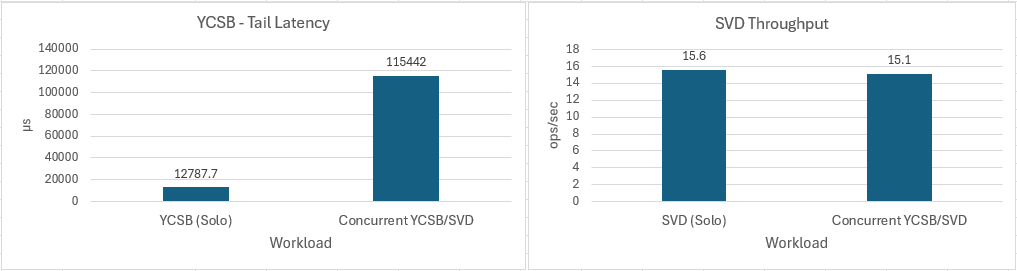
\includegraphics[scale=0.6]{images/nvm-motivation-sla.png}
  \caption[Performance Study]{Performance Study}
\end{figure}

\section{Architecture}

\begin{figure}[ht]
  \centering
  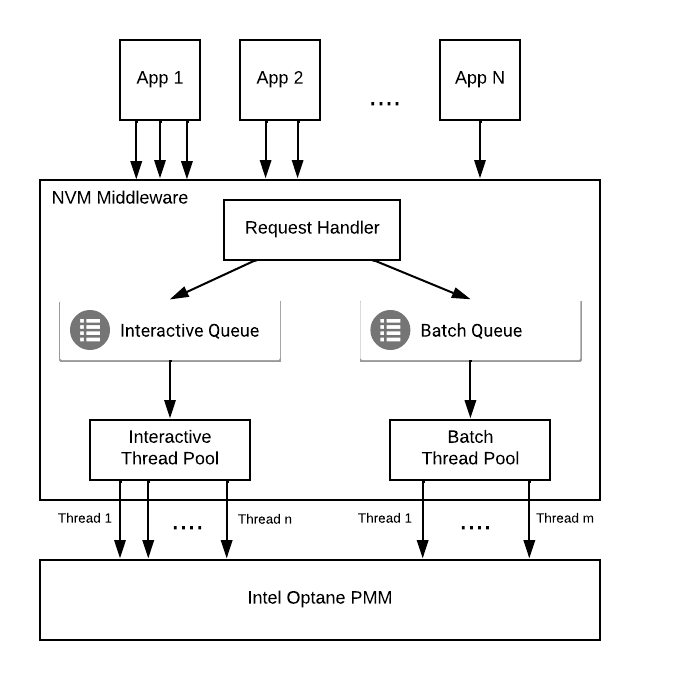
\includegraphics[scale=0.8]{images/nvm_design.png}
  \caption[NVM Middleware Architecture]{NVM Middleware Architecture}
\end{figure}

\section{Programming Interface}
Describe API here

\begin{table}[ht]
  \centering
  \caption{Programming Interface}
  % Tabular environment goes AFTER the caption!
  \begin{tabular}{|l|l|}
    % after \\: \hline or \cline{col1-col2} \cline{col3-col4} ...
    \hline
    \makecell{\textbf{API Name}} & \makecell{\textbf{Functionality}} \\
    \hline
    \rowcolor{gray!50} % Color the header row
    start(db, interactiveThreads, batchThreads) & \makecell[cl] {Creates PMEMKV database. \\ Start control threads.} \\
    close() & \makecell[cl] {Close PMEMKV database. \\ Stop all threads.} \\\hline
    \rowcolor{gray!50}
    get(key, mode) & Retrieves key from persistent memory. \\
    put(key, value, mode) & Writes key to persistent memory. \\
    \hline
  \end{tabular}
\end{table}

\section{Dynamic concurrency control with Reinforcement Learning}
Start section here

\begin{table}[ht]
  \centering
  \caption{The State Representation}% Color the header row
  % Tabular environment goes AFTER the caption!
  \begin{tabular}{|l|l|}
    % after \\: \hline or \cline{col1-col2} \cline{col3-col4} ...
    \hline
    \makecell{\textbf{Name}} & \makecell{\textbf{Description}} \\\hline
    \rowcolor{gray!50} % Color the header row
    interactiveThreads & Number of interactive threads. \\\hline
    batchThreads & Number of batch threads. \\\hline
    \rowcolor{gray!50} % Color the header row
    interactiveQueueSize & Interactive Queue Size. \\\hline
    batchQueueSize & Batch queue size. \\\hline
    \rowcolor{gray!50} % Color the header row
    interactiveBlockSize & Average block size of interactive workload. \\\hline
    batchaBlockSize & Average bloc size of batch workload. \\\hline
    \rowcolor{gray!50} % Color the header row
    interactiveRWRatio & Read/Write ratio of interactive workload. \\\hline
    batchRWRatio & Read/Write ratio of batch workload. \\
    \hline
  \end{tabular}
\end{table}

\begin{table}[ht]
  \centering
  \caption{The set of possible actions}
  % Tabular environment goes AFTER the caption!
  \begin{tabular}{|c|l|l|}
    % after \\: \hline or \cline{col1-col2} \cline{col3-col4} ...
    \hline
    \thead{Action} & $interactiveThreads_{t+1}$ & $batchThreads_{t+1}$ \\\hline
    0 & $interactiveThreads_{t+1}$ = $interactiveThreads_{t}$ & $batchThreads_{t+1}$ = $batchThreads_{t}$ \\\hline
    1 & $interactiveThreads_{t+1}$ = $interactiveThreads_{t}$ + 1 & $batchThreads_{t+1}$ = $batchThreads_{t}$ \\\hline
    2 & $interactiveThreads_{t+1}$ = $interactiveThreads_{t}$ - 1 & $batchThreads_{t+1}$ = $batchThreads_{t}$ \\\hline
    3 & $interactiveThreads_{t+1}$ = $interactiveThreads_{t}$ & $batchThreads_{t+1}$ = $batchThreads_{t}$ + 1 \\\hline
    4 & $interactiveThreads_{t+1}$ = $interactiveThreads_{t}$ & $batchThreads_{t+1}$ = $batchThreads_{t}$ -1 \\\hline
    5 & $interactiveThreads_{t+1}$ = $interactiveThreads_{t}$ + 1 & $batchThreads_{t+1}$ = $batchThreads_{t}$ + 1 \\\hline
    6 & $interactiveThreads_{t+1}$ = $interactiveThreads_{t}$ + 1 & $batchThreads_{t+1}$ = $batchThreads_{t}$ - 1 \\\hline
    7 & $interactiveThreads_{t+1}$ = $interactiveThreads_{t}$ - 1  & $batchThreads_{t+1}$ = $batchThreads_{t}$ + 1 \\\hline
    8 & $interactiveThreads_{t+1}$ = $interactiveThreads_{t}$ - 1  & $batchThreads_{t+1}$ = $batchThreads_{t}$ - 1 \\
    \hline
  \end{tabular}
\end{table}

\section{Implementation}